\documentclass{article}
\usepackage{graphicx}
\graphicspath{{./}}
\title{Project Proposal}
\author{Saahil Shihaz}
\date{November 12, 2021}
\begin{document}
\maketitle
\newpage
\section{Project Title}
Flower species recognition on a smartphone.
\section{Problem Description}
The technological era that we live in has introduced many ground breaking achievements that constantly push the barrier of what is possible as well as introduce many new challenges that require complex solutions. One such challenge is big data processing, specifically, recognising patterns in data and drawing conclusions. Unfortunately machines don’t have the ability to understand data the way that humans do and humans don’t have the processing capability of modern machines. Due to obvious ethical and biological barriers, we cannot make humans fill the role of computers that compute data on a large scale, therefore, we must explore the alternative, making computers as smart as humans. This is where machine learning steps in, with which we have made great advancements in. What this project will focus on in particular, is granting the advanced capabilities of machine learning to lower end hardware.
\\
\\
This project aims to investigate the application of machine learning techniques to recognize images of flowers species on mobile devices. I will look at implementing standard machine learning algorithms that are effective in image classification as well as alternative deep learning techniques which are more effective in carrying out the same task. It will be interesting to compare both types of implementations in terms of accuracy, speed and performance and then transferring them to a mobile hardware environment which is traditionally weaker than standard machines such as desktops and laptops. Ultimately, we want to understand the best way in making a mobile software solution that can make use of machine learning methods and still maintain a seamless user experience.
\\
\\
Mobile devices have the advantage of portability and flexibility compared to PCs at the expense of pure processing power, storage and battery life. Advancements in machine learning can boost the abilities of mobile devices by allowing them to make informed decisions to aid the user. Traditional algorithms can’t make decisions like “What is this flower?” without being cumbersome and inaccurate, we need something that can make good decisions and evolve, similar to human thinking. Smart phones and tablets are packed with more advanced technology than they’ve ever had like high resolution camera, sensors, displays and mobile processors, each of these are resources that a well written machine learning algorithm can take advantage of, for example, in our case, a mobile phone that can provide high resolution photos of flowers. The more detailed data we can use to aid our machine learning process, the better. 
\\
\\
Traditionally, mobile devices as well as similar devices with sensors do some light pre-processing of data, then they send it to the cloud which can handle actions that require intensive processing, this introduces some level of latency because of the communication between device and the cloud (Olascoaga, Meert and Verhelst, 2020, p. 3) \cite{Isabel}. Latency, being a key issue, is important in some use cases such as autonomous vehicles, mobile gaming, activity tracking for vulnerable populations, etc (Olascoaga, Meert and Verhelst, 2020, pp. 3-4) \cite{Isabel}.
\\
\\
With some raw information, a (classical) machine learning process can identify features, these could be used by a classifier that can make predictions given a set of data it hasn’t seen before (Lecun, Bengio and Hinton, 2015) \cite{LeCun}. Features are sourced from the representation of an object, in turn the representation is defined by the data input. An example of a feature would be the presence or absence of thorns on the stem of a flower (Goodfellow, Bengio and Courville, 2016, p. 22) \cite{Goodfellow}. Traditional machine learning practices incorporated feature engineering that required designing custom algorithms for particular task which can be time consuming (Liu, Lin and Maosung, 2020) \cite{Liu}. There is also difficulty in understanding what features should be extracted, for example, it may be hard to represent flower petal shapes properly from raw pixel values if there are shadows being cast on it (Goodfellow, Bengio and Courville, 2016, p. 23) \cite{Goodfellow}. Representation learning is a method that can fix such issues by providing mappings not from just the representation of data to the output, but from representation to representation (Goodfellow, Bengio and Courville, 2016, p. 24) \cite{Goodfellow}. There are however, still hurdles to overcome, these are described as “factors of variation” where external factors might affect the source data, such as, the age of a flower, which could affect the petal shape and the season which may affect a flower’s appearance. Factors like this make it difficult to get representations in the first place (Goodfellow, Bengio and Courville, 2016, p. 24) \cite{Goodfellow}.
\\
\\
Deep learning is a part of machine learning that aims to overcome limitations of classical machine learning techniques by expanding upon representation learning. Deep learning can be split into two unique parts: 
\begin{itemize}
    \item Distributed Representation: These are used to represent objects within a more compact and dense manner, instead of having representations for each type of object, for example a collection of words in a sentence, we could store the frequency of each word like the bag-of-words problem (Liu, Lin and Maosung, 2020) \cite{Liu}. This is a sparse representation and introduces problems with space and time complexity. Therefore distributed representations aim to tackle the sparsity problem as they are harder to model (Brownlee, 2017) \cite{Brownlee}.
    \item Deep Architecture: The idea of layering to represent neurons in a human brain. You can imagine it as a map of nodes that takes an input, processes it through the different layers where at each step, a set of units calculate a weighted sum of their inputs from the previous layer and pass the result to the next layer until it gets to output units that generate a result. This is an example of a feedforward neural network (Lecun, Bengio and Hinton, 2015) \cite{LeCun}.
\end{itemize}
Input into a deep learning algorithm starts at the visible layer, which contains our set of input pixels that we can directly observe. This data is passed into a network of hidden layers, each of these layers represent an abstract feature that we can’t normally observe by looking at the input data such as locations of edges and contours (Goodfellow, Bengio and Courville, 2016, p. 26) \cite{Goodfellow}.
\\
\\
By making use of TensorFlow (Lite) we can produce classification models using languages like Python, C++ or Java, then convert said models into small packages that an Android/IOS application can use to generate predictions based on an input. TensorFlow is developed by Google and provides an machine learning based suite of tools to design, test and deploy ML solutions. The Lite version that we will be using is designed specifically for mobile devices and IoT devices that may not have the support of powerful hardware. Using TensorFlow we can write models that use classical ML techniques as well as deep learning techniques like Convolutional Neural Networks (CNN) (Google, n.d.) \cite{Google}. There are examples that can be built specifically for flower classification within the API documentation which can serve as a starting point for the project.
\section{Existing Solutions}
\subsection{Pl@ntNet}
This app generates predictions using it’s extremely large database of flora separated into a large amount categories based on theme and location. There are also users who can contribute images to help refine predictions. A user has to choose a relevant category like the location to help with the prediction. There is also an API that allows for developers to use the same functionality.
\subsection{iNaturalist}
A learning tool that relies on crowdsourcing to gather images about nature, it uses experts to identify observations rather than a machine. There is heavy emphasis on social media and gathering communities of people interested in observations of nature.
\subsection{PlantSnap}
Identifies plants using an image and provides information related to the plant like facts and how to take care of it. You can also have a profile where you show the plants that you have taken pictures of as part of your collection. 
\subsection{Review}
There are many more solutions for flower and plant identification, each providing unique ways in carrying out the identification process. There are many that describe themselves using “AI” techniques to identifying objects, but do not expand further than that. We can also see that ML is not necessarily the only method of identification and that crowdsourcing is still viable. A unique take on the flower identification process might be to expose that various ML techniques used in identification rather than abstracting it like these existing systems do.
\section{Main Objectives}
\begin{itemize}
    \item Analyse existing mobile based image recognition software.
    \item Investigate the advantages and disadvantages of both classical ML and DL implementations and compare the two using analysis tools, this will be done on PC hardware.
    \item Design and engineer an Android application that can recognize images using the ML implementation that we determine as the best.
    \item Explore future improvements for the Android app.
\end{itemize}
\section{High Level Requirements}
In order to expand on what the main objectives of the project, I will provide requirements that are musts for this project to succeed as well as potential requirements that the project could explore.
\subsection{Functional Requirements}
\begin{itemize}
    \item Must be able to demonstrate a working solution that can recognize different species of flowers using classical machine learning.
    \item Must be able to demonstrate which classical method is best in by analysing performance and accuracy.
    \item Must be able to demonstrate a working solution that can recognize different species of flowers using deep learning.
    \item Must be able to demonstrate which deep learning method is best by analysing performance and accuracy.
    \item Must be able to demonstrate the best implementation of ML that is found inside an Android application.
\end{itemize}
\subsection{Non-functional Requirements}
\begin{itemize}
    \item The implementation must function correctly with minimal bugs in order to fairly compare all solutions.
    \item The same hardware and software must be used to demonstrate and compare all solutions.
    \item The project must detail any implementation, code and algorithms that are not the original work of me, such as the use of open source software.
    \item The project must be backed up and maintained properly using version control and cloud based services.
    \item The application should be simple to use for non-technical users and work with minimal bugs.
    \item The project could explore possible improvements to the application in general to improve usability and increase usefulness of the solution.
\end{itemize}
\section{Project Plan}
The Gantt chart in figure 1 outlines a general structure for the project, mainly using the major hand in milestones to split each section. I have included time to review first drafts with my supervisor so that we can discuss feedback and improvements before the hand in date. The chart will increase in detail over the lifetime of the project in order to make the overall plan more granular. I have combined some areas like the development of both solution types as it is likely a lot of development of one solution will overlap with another solution. What will also need to be added, likely after the demonstration of progress, is key dissertation milestones. I will discuss with my supervisor closer to the time what parts of the dissertation should be completed and when over the last period of time.
\\
\begin{figure}[h]
    
    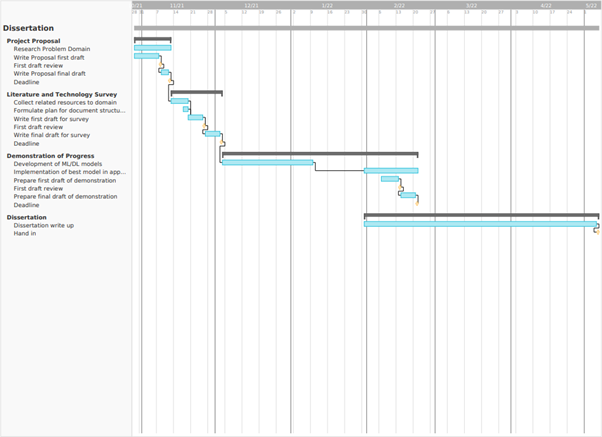
\includegraphics[width=\textwidth]{Gantt_Chart.png}
    \caption{Gantt Chart}
\end{figure}
\\
I believe that the period of mid-December to mid-February is enough for development, there is plenty of documentation for TensorFlow and tutorials to get started, therefore this period should go smoothly, however, there is plenty of time after the demonstration of progress to conduct further development if I feel it will be beneficial for the project overall. Each section is a suggestion and can be subject to change (apart from non-formative deadline milestones) depending on other commitments like exams and coursework for other modules. Therefore, each section should be treated as a period of time for when related tasked should be carried out within. Dissertation writing has some overlap with development and formally begins on the 31st of January as that is right after the semester one exam period where nothing is scheduled in on the Gantt chart. It is possible that phase two of development, which includes implementing the best solution on mobile could start earlier or later depending on how well phase one goes where I explore the ML and DL algorithms on my machine as well as the demonstration of progress deadline where I may need to actively work on that instead. Ideally I can get a working app solution as part of my demonstration of progress, therefore there is some overlap as shown on the chart.
\section{Resources}
\subsection{Literature}
Literature resources will be sourced online and will mainly consist of Journal articles, books, scientific papers and reliable webpages. These sources will be mainly found through the University of Bath online library and other repositories of the same nature.
API documentation, specifically for Android development and TensorFlow will be provided by Google Developers.
\subsection{Technology}
The project will be written and maintained using my personal PC hardware (Dell Inspiron 7591). This includes writing, communication and development. Writing the ML solutions will be done in Python with references to the TensorFlow API and Jupyter notebook software. The language that will be used is Java, using the Android Studio IDE to develop and deploy applications. I will be using my personal smartphone (Samsung Galaxy S20) in development mode to test and analyse all application solutions I will generate during the development lifecycle. Version control using Git and GitHub will be used to backup and maintain the codebase, it will be hosted within my private repository in my personal account. All project files will be backed up automatically to the cloud using Microsoft OneDrive.
\subsection{Data}
All data resources will be sourced online, fortunately there are many data sets that are split into categories that will be useful for training. All data resources that are used will be correctly referenced and credited.
\begin{thebibliography}{1}
\bibitem{Brownlee}
Brownlee, J., 2017. \textit{A Gentle Introduction to the Bag-of-Words Model}. [Online] Available from: https://machinelearningmastery.com/gentle-introduction-bag-words-model/ [Accessed 6 November 2021].
\bibitem{Goodfellow}
Goodfellow, I., Bengio, Y. \& Courville, A., 2016. \textit{Deep Learning}. Cambridge, Massachusetts: MIT Press
\bibitem{Google}
Google, n.d. Overview. [Online] Available at: https://www.tensorflow.org/lite [Accessed 5 November 2021].
\bibitem{Isabel}
Isabel Galindez Olascoaga, L., Meert, W. \& Verhelst, M., 2020. \textit{Hardware-Aware Probabilistc Machine Learning Models}. Switzerland: Springer.
\bibitem{LeCun}
LeCun, Y., Bengio, Y. \& Hinton, G., 2015. \textit{Deep Learning}. Nature, 521, pp. 436-444.
\bibitem{Liu}
Liu, Z., Lin, Y. \& Maosung, S., 2020. \textit{Representation Learning for Natural Language Processing}. New York: Springer.
\end{thebibliography}
\end{document}